\documentclass[11pt,a4paper]{article}

\usepackage[parfill]{parskip}
\usepackage{subfig}
\usepackage{amsmath}
\usepackage{makeidx}
\usepackage{graphicx}
\usepackage[bibstyle=numeric, citestyle=numeric-comp]{biblatex}
\usepackage{multicol}
\usepackage{letltxmacro}

%\addbibresource[location=remote]{C:/Users/CptProton/Documents/Bibliographies/Labs.bib}

\LetLtxMacro{\oldsqrt}{\sqrt} % makes all sqrts closed
\renewcommand{\sqrt}[1][]{%
  \def\DHLindex{#1}\mathpalette\DHLhksqrt}
\def\DHLhksqrt#1#2{%
  \setbox0=\hbox{$#1\oldsqrt[\DHLindex]{#2\,}$}\dimen0=\ht0
  \advance\dimen0-0.2\ht0
  \setbox2=\hbox{\vrule height\ht0 depth -\dimen0}%
  {\box0\lower0.71pt\box2}}

\makeatletter
\newenvironment{tablehere}
  {\def\@captype{table}}
  {}

\newenvironment{figurehere}
  {\def\@captype{figure}}
  {}
\makeatother

\title{Automatic Fingerprint Recognition}
\author{Benjamin May \& Edward Wastell}
%\date{}

\begin{document}
\maketitle

\begin{abstract}
Stuff happened.
\end{abstract}

\begin{multicols}{2}

\section{Introduction}
	Fingerprints have been used to identify people since the 19\textsuperscript{th} century and have been used in criminal investigations since about that time. More recently fingerprints have been used as biometric markers used in boarder control, library stock control and computer and building access control systems. The need for a robust automatic fingerprint recognition system is obvious.

	Most fingerprint recognition systems in use are based on the idea of identifying minutiae (points where a ridge ends or joins with another ridge) --- in this article a system that uses the greylevel gradient to find minutiae is discussed.

\section{Theory and Implementation}

	\subsection{Point Normal Direction}
\begin{figure*}
\centering
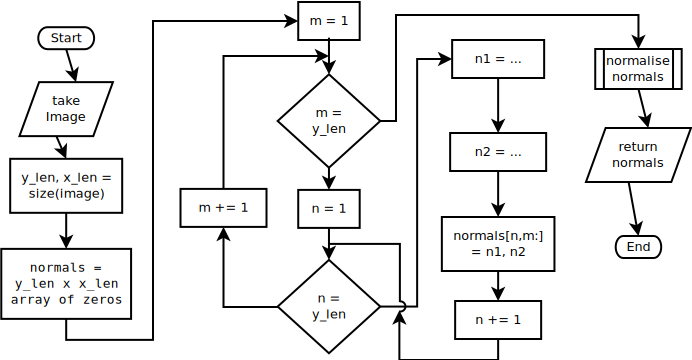
\includegraphics[width = \textwidth]{PND}
\caption{Flow chart of the PND function as implemented.}
\label{fig:PND-alg}
\end{figure*}

		The point normal function works by taking four mutually adjacent points (\textit{i.e.} a $2 \times 2$ array of pixels) and fitting a plane to them. If the greylevel at the pixel $(x_k, y_k)$ is denoted $h_k$ and the level from the fitted plane is denoted $p_k$ then the plane fitting part of the function can be seen as minimising the following expression:

		\begin{equation}
			\min_{n_1, n_2, c} \sum_k |h_k - p_k|^2
		\end{equation}
		
		Which in matrix form can be expresed as:

		\begin{equation}
			\begin{vmatrix}
			\begin{pmatrix}
			h_1 \\
			h_2 \\
			h_3 \\
			h_4
			\end{pmatrix}
			-
			\begin{pmatrix}
			-x_1 & -y_1 & 1 \\
			-x_2 & -y_2 & 1 \\
			-x_3 & -y_3 & 1 \\
			-x_4 & -y_4 & 1
			\end{pmatrix}
			\begin{pmatrix}
			n_1 \\
			n_2 \\
			c
			\end{pmatrix}
			\end{vmatrix}^2
		\end{equation}

		Where $n_1$, $n_2$ and $c$ are the $x$, $y$ and $z$ components of the surface normal respectively. This is a simple least-squares minimisation and after some rearranging we obtain the following expressions for the optimum surface normal:

		\begin{equation}
		\begin{split}
			n_1 = \frac{-h_1 + h_2 + h_3 - h_4}{4} \\
			n_2 = \frac{-h_1 - h_2 + h_3 + h_4}{4} \\
			c = \frac{h_1 + h_2 + h_3 + h_4}{4}
		\end{split}
		\end{equation}

		Since we are only concerned with the components in the $x,y$--plane the function implemented here doesn't bother calculating $c$ (figure \ref{fig:PND-alg}). Once all $2 \times 2$ neighbourhoods have been fitted the function returns $n_1$ and $n_2$ then terminates.

		As the NPD function needs a four points to fit a plane to the decision has to be made regarding how edges are handled. One possibility is to `wrap' the edges of the image around, effectivly forming a torus --- this was not implemented here because it would mean that for two edges the values of $n_1$ and $n_2$ would depend on greylevels from the other two edges. The second possibility (implemented here) is to make the output array smaller by 1 pixel in both dimensions, so if the original image is $n \times m$ pixels the array of normals is $(n-1) \times (m-1)$. From figure \ref{fig:PND-alg} it can be seen that the PND function implemented here loses the top and right hand pixels.

	\subsection{Averaged Tangent Direction}
		The ATD function calcualtes the $x,y$--plane tangent that best fits with the surface normals generated by the PND function in a given $n \times n$ neighbourhood. This has the effect of smoothing out (plane normal angle) noise but, as with analogous smoothing operations, can obscure features with a size comprable to that of the kernel chosen. Here a default kernel of size $9 \times 9$ is chosen, which should balance computation time and over smoothing against noise correction.

		

\section{Experimental Procedure}

\section{Results \& Analysis}

\section{Conclusion}


\printbibliography

\end{multicols}

\end{document}
